\documentclass[../main.tex]{subfiles}

\begin{document}

\section{Actions and Energy}

During a unit’s activation, that unit can use its Energy stat to complete unique Actions before, during, or after using its Movement. All Actions require one Energy to use and cannot be performed more than once per turn by the same unit. Some Actions need a D20 roll of 10+ to be successful.

\textit{Note: The same Action cannot be done multiple times by the same unit during a turn. For example, a single unit with three Energy cannot Mine three times. But a Character with four different units that each have one Energy could Mine with each of those units when activating them during the same turn. This is what makes multi-unit Characters strong gatherers.}

Below is a list of the different Actions units can take during their activation.

\subsection{Action: Fish}
The Fish Action allows units to catch fish from the water that can heal, cleanse, and buff Characters. With a little bit of luck, fishing can also provide valuable treasures.

\subsubsection{How to Fish? }
If a non-engaged unit on a land hex is adjacent to an unoccupied water tile that is lower than the unit’s base, the unit may use 1 Energy to perform the Fish Action and roll a D20. On a successful roll (10+), the player will draw one fish card and place it in the inventory of the active Character. Tamed Monsters cannot perform the Fish Action.

\centering
    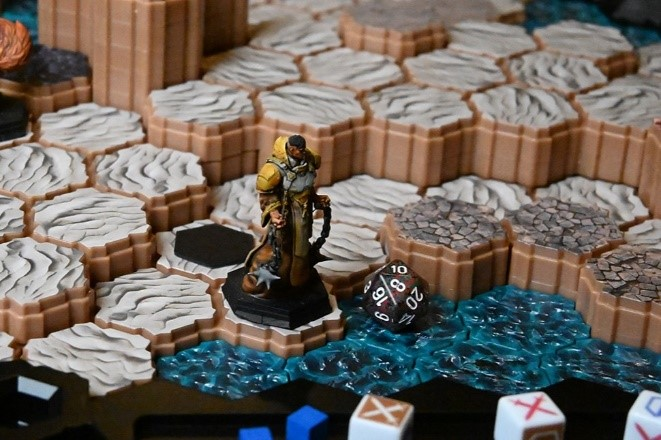
\includegraphics[width=1\linewidth]{chapters//ActionsandEnergy/TimeStrikeCharFishing.jpg}  

\textit{Image: Character adjacent to water successfully rolls to draw a fish card.}

\subsection{Action: Mine}
The Mine Action allows units to collect materials that are used for building roads and walls.
\subsubsection{How to Mine? }
If a non-engaged unit is adjacent to an unoccupied resource hex, it may use 1 Energy to perform the Mine Action and collect one material. Take the resource hex and place it in the inventory of the Character that performed the Mine Action. Resource hexes that are in a Character’s inventory are referred to as materials. Tamed Monsters cannot perform the Mine Action.
\centering
    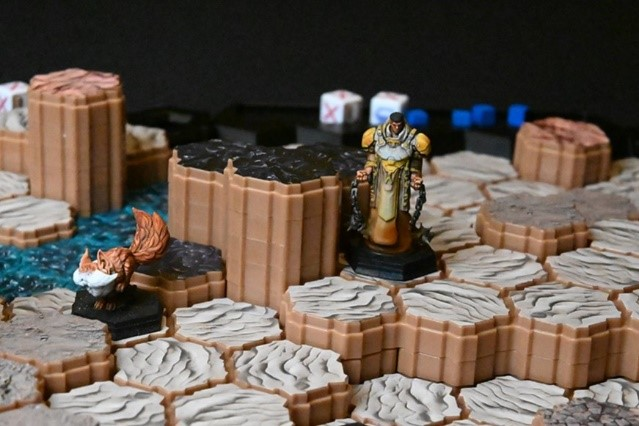
\includegraphics[width=1\linewidth]{chapters//ActionsandEnergy/TimeStrikeCharMine1.jpg} 
Image: Character adjacent to a resource hex. 

\centering
    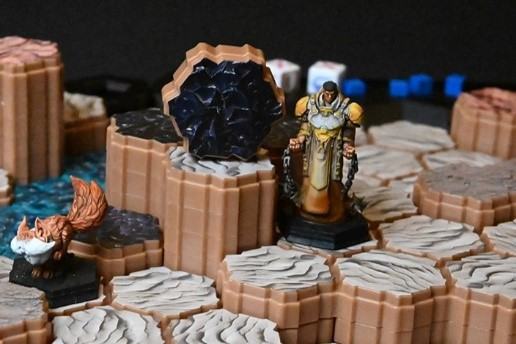
\includegraphics[width=1\linewidth]{chapters//ActionsandEnergy/TimeStrikeCharMine2.jpg}  
Image: Character picking up a material. 

\subsection{Action: Trade}
The Trade Action allows units to exchange various goods between allied Characters. Materials, fish, and loot cards are all considered to be goods.

\subsubsection{How to Trade? }
A non-engaged unit can use 1 Energy to perform the Trade Action with an adjacent allied Character that is also non-engaged. Both Characters involved in the trade may each transfer up to 1 good from their inventory to the other Character’s inventory. A Character may both give and receive goods during a single Trade Action. Tamed Monsters cannot perform the Trade Action.

\subsection{Action: Climb Sentience}
Each Sentience has multiple tiers which can be climbed by units. While on the Sentience, units can attack the Sentience as well as other units on the Sentience. In addition, units that climb the Sentience cannot be targeted by units (whether friendly or enemy) that are not on the Sentience, and cannot target units that are not on the Sentience. (see the rules for Targeting). 

\subsubsection{How to Climb the Sentience?}
If a unit is adjacent to or on the Sentience it may use 1 Energy to perform the Climb Sentience Action, allowing the unit to climb up to the next highest tier of the Sentience if that tier is unoccupied.
\centering
    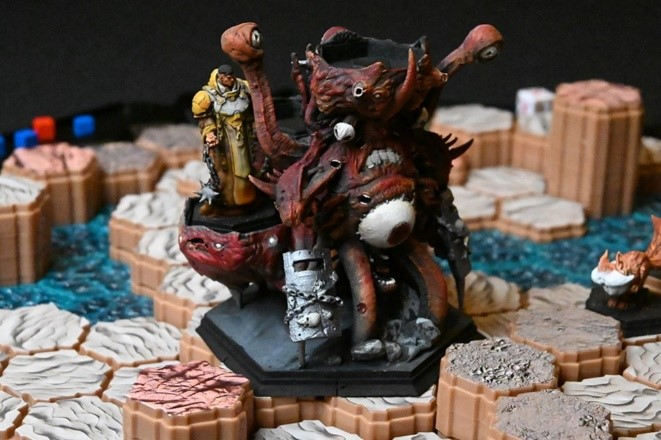
\includegraphics[width=1\linewidth]{chapters//ActionsandEnergy/TimeStrikeClimbSentience.jpg}
\textit{Image: Character climbing up a tier on the Sentience.}

Units that are on the Sentience already can instead use the Climb Sentience Action to be placed on any unoccupied hex adjacent to the Sentience

\textit{Note: Units do not take fall damage when knocked off the Sentience.}

\subsection{Action: Contest}
The Contest Action allows units to challenge other units for positioning. Contests can result in swapping positions with the opposing unit or pushing the opposing unit off their hex to an adjacent hex of the contestant’s choosing if they are victorious. Contesting can be used to push enemies off high elevations, swap positions to take over the high ground, or simply to assert dominance.

\subsubsection{How to Contest? }
If a unit is adjacent to an opponent’s unit, it may use 1 Energy to perform the Contest Action against one of those units. Units do not necessarily have to be engaged to contest one another. During a contest, both players roll 1D20, and the action is successful if the active unit rolls higher than the contested unit.

\textit{Note: Ties are rewarded to the Defender.}

\centering
    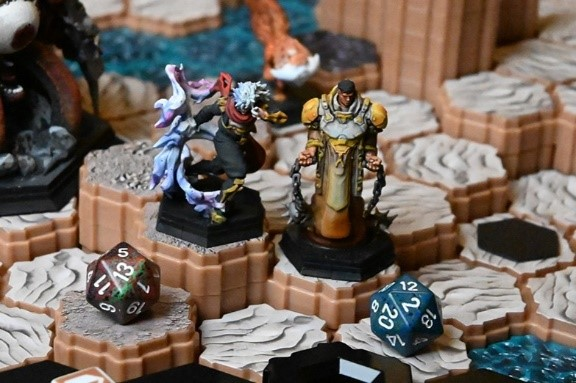
\includegraphics[width=1\linewidth]{chapters//ActionsandEnergy/TimeStrikeContesting.jpg}

\textit{Image: Two units contesting with the lower unit rolling higher.}

If the Contest Action is successful, the active player can switch the positions of the two units. 

If the units were engaged, the active player can instead choose to push the opponent’s unit by moving it one hex in any direction that is lower than or equal to the contested unit’s position.

Units that are pushed or switched by a successful Contest Action are subject to fall damage. Since the Contest Action does not use the unit’s Movement stat, units moved by the Contest Action never receive Cheap Shots.

\centering
    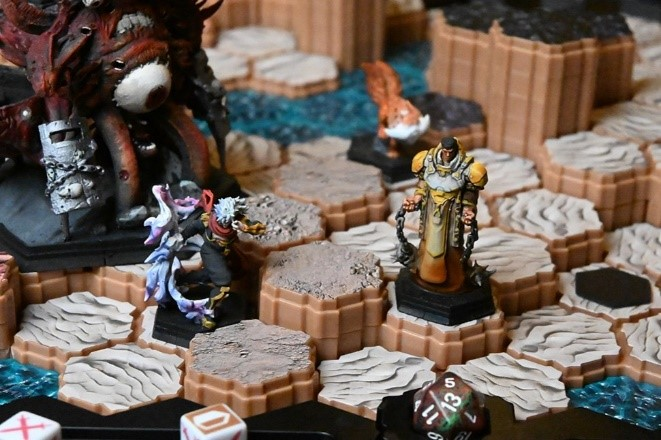
\includegraphics[width=1\linewidth]{chapters//ActionsandEnergy/TimeStrikeWinningContest.jpg} 

\textit{Image: Winning contester pushing the unit 1 hex.}

\centering
    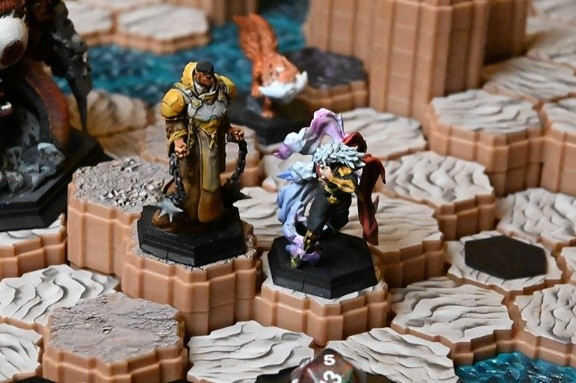
\includegraphics[width=1\linewidth]{chapters//ActionsandEnergy/TimeStrikeContestSwapping.jpg}

\textit{Image: Winning contester swapping positions with the unit.}

\subsubsection{Contesting Different Size Units}'
Units can only Contest units with an equal or lower hex size. A 1-hex unit cannot Contest a 2-hex unit. A 2-hex unit cannot Contest a 3-hex unit, and so on.

\subsubsection{Contesting Upwards}
If the contested unit’s base is on a higher level elevation than the active unit’s base and the two units are not engaged with each other, the contested unit adds 5 to their die roll.

\subsubsection{Contesting Down}
A unit may not Contest a unit on a lower elevation unless they are engaged with that unit.

\subsubsection{Contesting on the Sentience}
Units can also Contest each other for positions on the Sentience. A unit on a tier of the Sentience can Contest another unit on an adjacent tier of the Sentience. If successful, the contester may either switch positions with the contested unit, or place the contested unit on any unoccupied space adjacent to the Sentience.

A unit on a hex adjacent to the Sentience can Contest a unit on the first tier to switch positions with them. In this case, the contested unit always adds 5 to their roll.

\subsection{Action: Tame Monster}
The Tame Monster Action is an attempt to control a Lost Monster and add it to your team. Failing to tame a Monster, however, will result in taking damage.
\textit{Note: Only Survivors may tame Monsters. Monsters cannot tame other Monsters.}

\subsection{How to Tame Monster? }
If a Survivor unit is engaged with a Lost Monster the unit can try to tame it. The Monster will attack the unit trying to tame it equal to the “Lost Attack” stat on the Sentience card. Roll the unit’s Defense. If the taming unit blocks the entire attack, the tame is successful. Otherwise, the unit takes any unblocked damage and the tame fails.

\textit{Note: Height advantage and other modifiers are considered when defending against an attack while taming.}

If a Beast is successfully tamed, place its Character card next to the Character card of the unit that tamed it. The tamed Beast can now be activated when taking a turn with the Character that tamed it. This effectively allows you to activate multiple units during a single turn. 

If a Brute is successfully tamed, place the unit that tamed the Brute into the mount slot on top of the Brute. The two units are now referred to collectively as a Behemoth and are subject to special rules. (See the “Tamed Brute” section for the rules.)

\subsection{Action: Cast Ability}
The Cast Ability Action allows units to use an ability type skill on their Character card.

\subsubsection{How to Cast Ability?}
If a unit’s Character card contains a skill labeled as “Ability”, that unit can spend 1 Energy to perform the Cast Ability Action and use the ability.

\subsection{Action: Attack}
The Attack Action allows units to attempt to damage the units of other players or the Lost. Any unit can target and attack another unit by using the attacking unit’s Range and Attack stats. After performing the Attack Action, the active unit may no longer use their Movement or use their Energy to take additional actions for the remainder of the turn. Learn more about targeting and attacking in the following section: “Targeting and Combat.”

\clearpage
\end{document}